\documentclass{article}
\usepackage{amsmath}
\usepackage{amssymb}
\usepackage{geometry}
\usepackage{graphicx} % For including images
\usepackage{tikz} % For creating diagrams
\usepackage{pgfplots} % For creating diagrams
\pgfplotsset{compat=1.18} % Set pgfplots compatibility mode
\geometry{a4paper, margin=1in}

\begin{document}


\section*{Local Linear and Quadratic Approximations of a Function}

To find and use local linear and local quadratic approximations of a function \( f(x) \) at \( x = x_0 \), follow these steps:

\subsection*{Local Linear Approximation (Tangent Line Approximation)}
The local linear approximation of \( f(x) \) at \( x = x_0 \) is given by the equation of the tangent line to the function at that point. This can be expressed as:
\[ L(x) = f(x_0) + f'(x_0)(x - x_0) \]
where:
\begin{itemize}
\item \( f(x_0) \) is the value of the function at \( x = x_0 \).
\item \( f'(x_0) \) is the derivative of the function at \( x = x_0 \).
\end{itemize}

\begin{center}
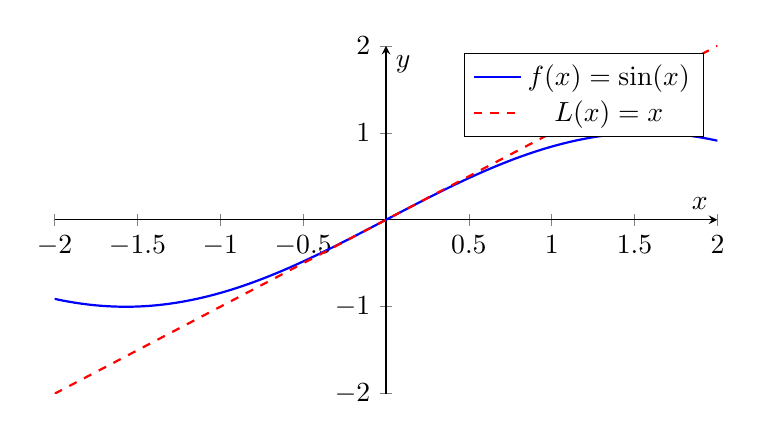
\begin{tikzpicture}
\begin{axis}[
    axis lines = middle,
    xlabel = \(x\),
    ylabel = \(y\),
    domain=-2:2,
    samples=100,
    width=10cm,
    height=6cm,
]
\addplot [blue, thick] {sin(deg(x))};
\addplot [red, thick, dashed] {x};
\legend{\(f(x) = \sin(x)\), \(L(x) = x\)}
\end{axis}
\end{tikzpicture}
\end{center}

\subsubsection*{Steps to Find the Local Linear Approximation}
\begin{enumerate}
\item Compute \( f(x_0) \).
\item Compute \( f'(x_0) \).
\item Substitute \( f(x_0) \) and \( f'(x_0) \) into the linear approximation formula \( L(x) = f(x_0) + f'(x_0)(x - x_0) \).
\end{enumerate}

\subsection*{Local Quadratic Approximation (Second-Order Taylor Polynomial)}
The local quadratic approximation of \( f(x) \) at \( x = x_0 \) includes terms up to the second derivative of the function and is given by:
\[ Q(x) = f(x_0) + f'(x_0)(x - x_0) + \frac{f''(x_0)}{2}(x - x_0)^2 \]
where:
\begin{itemize}
\item \( f(x_0) \) is the value of the function at \( x = x_0 \).
\item \( f'(x_0) \) is the first derivative of the function at \( x = x_0 \).
\item \( f''(x_0) \) is the second derivative of the function at \( x = x_0 \).
\end{itemize}

\begin{center}
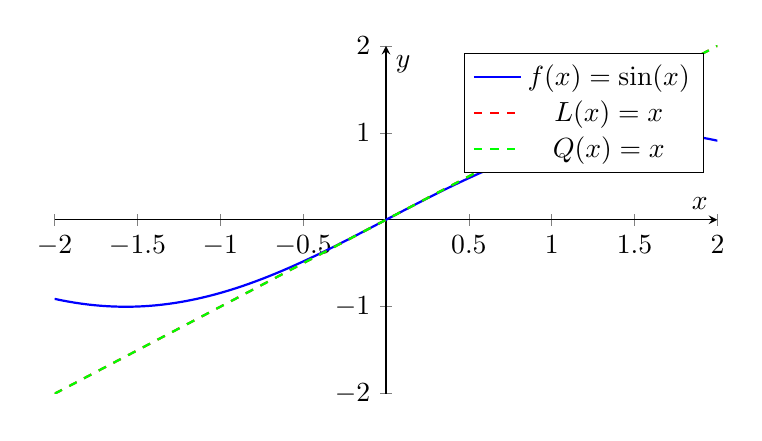
\begin{tikzpicture}
\begin{axis}[
    axis lines = middle,
    xlabel = \(x\),
    ylabel = \(y\),
    domain=-2:2,
    samples=100,
    width=10cm,
    height=6cm,
]
\addplot [blue, thick] {sin(deg(x))};
\addplot [red, thick, dashed] {x};
\addplot [green, thick, dashed] {x};
\legend{\(f(x) = \sin(x)\), \(L(x) = x\), \(Q(x) = x\)}
\end{axis}
\end{tikzpicture}
\end{center}

\subsubsection*{Steps to Find the Local Quadratic Approximation}
\begin{enumerate}
\item Compute \( f(x_0) \).
\item Compute \( f'(x_0) \).
\item Compute \( f''(x_0) \).
\item Substitute \( f(x_0) \), \( f'(x_0) \), and \( f''(x_0) \) into the quadratic approximation formula \( Q(x) = f(x_0) + f'(x_0)(x - x_0) + \frac{f''(x_0)}{2}(x - x_0)^2 \).
\end{enumerate}

\subsection*{Usage of Local Approximations}
Local approximations are useful for estimating the value of a function near a point \( x = x_0 \) without needing the exact form of the function. The linear approximation provides a quick estimate, while the quadratic approximation offers a more accurate estimate by considering the curvature of the function.

\subsubsection*{Example}
Suppose \( f(x) = \sin(x) \) and we want to approximate it near \( x_0 = 0 \):
\begin{enumerate}
\item \( f(0) = \sin(0) = 0 \)
\item \( f'(0) = \cos(0) = 1 \)
\item \( f''(0) = -\sin(0) = 0 \)
\end{enumerate}

The local linear approximation at \( x = 0 \) is:
\[ L(x) = 0 + 1 \cdot (x - 0) = x \]

The local quadratic approximation at \( x = 0 \) is:
\[ Q(x) = 0 + 1 \cdot (x - 0) + \frac{0}{2}(x - 0)^2 = x \]

In this case, both the linear and quadratic approximations are the same because the second derivative at \( x = 0 \) is zero.

\subsection*{Maclaurin Polynomials}
Maclaurin polynomials are a special case of Taylor polynomials centered at \( x = 0 \). They provide an approximation of a function \( f(x) \) near \( x = 0 \) using a polynomial whose coefficients are derived from the derivatives of \( f(x) \) at \( x = 0 \).

\subsubsection*{Theory}
The Maclaurin polynomial of degree \( n \) for a function \( f(x) \) is given by:
\[ P_n(x) = f(0) + f'(0)x + \frac{f''(0)}{2!}x^2 + \frac{f'''(0)}{3!}x^3 + \cdots + \frac{f^{(n)}(0)}{n!}x^n \]
This polynomial is constructed by taking the first \( n \) terms of the Maclaurin series expansion of \( f(x) \) around \( x = 0 \). The general form of the Maclaurin series for \( f(x) \) is:
\[ f(x) = \sum_{k=0}^{\infty} \frac{f^{(k)}(0)}{k!} x^k \]

\subsubsection*{Steps to Determine the Maclaurin Polynomial}
\begin{enumerate}
\item Compute \( f(0) \).
\item Compute \( f'(0) \).
\item Compute \( f''(0) \).
\item Continue computing higher-order derivatives at \( x = 0 \) up to \( f^{(n)}(0) \).
\item Substitute these values into the Maclaurin polynomial formula.
\end{enumerate}

\subsubsection*{Sigma Notation for the n-th Maclaurin Polynomial}
The \( n \)-th Maclaurin polynomial can be compactly written using sigma notation as:
\[ P_n(x) = \sum_{k=0}^{n} \frac{f^{(k)}(0)}{k!} x^k \]

\subsubsection*{Example}
Suppose \( f(x) = e^x \) and we want to find the Maclaurin polynomials of various degrees:
\begin{enumerate}
\item \( f(0) = e^0 = 1 \)
\item \( f'(0) = e^0 = 1 \)
\item \( f''(0) = e^0 = 1 \)
\item \( f'''(0) = e^0 = 1 \)
\item Continue this pattern for higher-order derivatives.
\end{enumerate}

The Maclaurin polynomials for \( f(x) = e^x \) are:
\begin{itemize}
\item \( P_0(x) = 1 \)
\item \( P_1(x) = 1 + x \)
\item \( P_2(x) = 1 + x + \frac{x^2}{2!} \)
\item \( P_3(x) = 1 + x + \frac{x^2}{2!} + \frac{x^3}{3!} \)
\item And so on.
\end{itemize}

Using sigma notation, the \( n \)-th Maclaurin polynomial for \( f(x) = e^x \) is:
\[ P_n(x) = \sum_{k=0}^{n} \frac{f^{(k)}(0)}{k!} x^k = \sum_{k=0}^{n} \frac{x^k}{k!} \]

\begin{center}
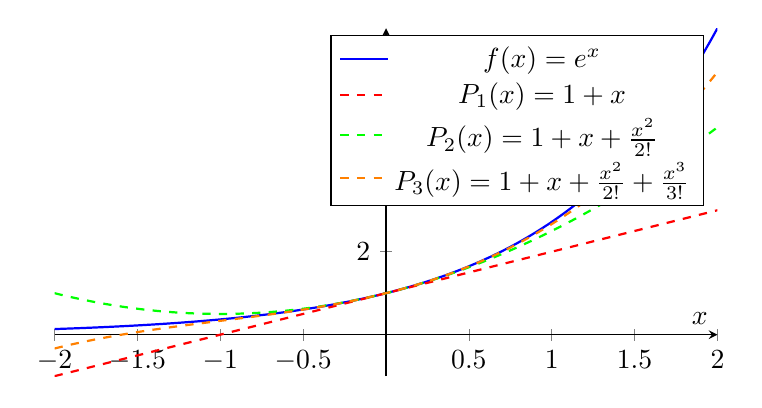
\begin{tikzpicture}
\begin{axis}[
    axis lines = middle,
    xlabel = \(x\),
    ylabel = \(y\),
    domain=-2:2,
    samples=100,
    width=10cm,
    height=6cm,
]
\addplot [blue, thick] {exp(x)};
\addplot [red, thick, dashed] {1 + x};
\addplot [green, thick, dashed] {1 + x + x^2/2};
\addplot [orange, thick, dashed] {1 + x + x^2/2 + x^3/6};
\legend{\(f(x) = e^x\), \(P_1(x) = 1 + x\), \(P_2(x) = 1 + x + \frac{x^2}{2!}\), \(P_3(x) = 1 + x + \frac{x^2}{2!} + \frac{x^3}{3!}\)}
\end{axis}
\end{tikzpicture}
\end{center}

\subsection*{Taylor Polynomials}
The Taylor polynomial provides an approximation of a function \( f(x) \) near a specified point \( x = x_0 \) using a polynomial whose coefficients are derived from the derivatives of \( f(x) \) at \( x = x_0 \).

\subsubsection*{Theory}
The Taylor polynomial of degree \( n \) for a function \( f(x) \) centered at \( x = x_0 \) is given by:
\[ P_n(x) = f(x_0) + f'(x_0)(x - x_0) + \frac{f''(x_0)}{2!}(x - x_0)^2 + \frac{f'''(x_0)}{3!}(x - x_0)^3 + \cdots + \frac{f^{(n)}(x_0)}{n!}(x - x_0)^n \]
This polynomial is constructed by taking the first \( n \) terms of the Taylor series expansion of \( f(x) \) around \( x = x_0 \). The general form of the Taylor series for \( f(x) \) around \( x = x_0 \) is:
\[ f(x) = \sum_{k=0}^{\infty} \frac{f^{(k)}(x_0)}{k!} (x - x_0)^k \]

\subsubsection*{Steps to Determine the Taylor Polynomial}
\begin{enumerate}
\item Compute \( f(x_0) \).
\item Compute \( f'(x_0) \).
\item Compute \( f''(x_0) \).
\item Continue computing higher-order derivatives at \( x = x_0 \) up to \( f^{(n)}(x_0) \).
\item Substitute these values into the Taylor polynomial formula.
\end{enumerate}

\subsubsection*{Sigma Notation for the n-th Taylor Polynomial}
The \( n \)-th Taylor polynomial can be compactly written using sigma notation as:
\[ P_n(x) = \sum_{k=0}^{n} \frac{f^{(k)}(x_0)}{k!} (x - x_0)^k \]

\subsubsection*{Example}
Suppose \( f(x) = \cos(x) \) and we want to find the Taylor polynomials of various degrees centered at \( x_0 = 0 \):
\begin{enumerate}
\item \( f(0) = \cos(0) = 1 \)
\item \( f'(0) = -\sin(0) = 0 \)
\item \( f''(0) = -\cos(0) = -1 \)
\item \( f'''(0) = \sin(0) = 0 \)
\item Continue this pattern for higher-order derivatives.
\end{enumerate}

The Taylor polynomials for \( f(x) = \cos(x) \) centered at \( x_0 = 0 \) are:
\begin{itemize}
\item \( P_0(x) = 1 \)
\item \( P_1(x) = 1 \) (since the first derivative term is zero)
\item \( P_2(x) = 1 - \frac{x^2}{2!} \)
\item \( P_3(x) = 1 - \frac{x^2}{2!} \) (since the third derivative term is zero)
\item And so on.
\end{itemize}

Using sigma notation, the \( n \)-th Taylor polynomial for \( f(x) = \cos(x) \) centered at \( x_0 = 0 \) is:
\[ P_n(x) = \sum_{k=0}^{n} \frac{f^{(k)}(0)}{k!} x^k \]

\begin{center}
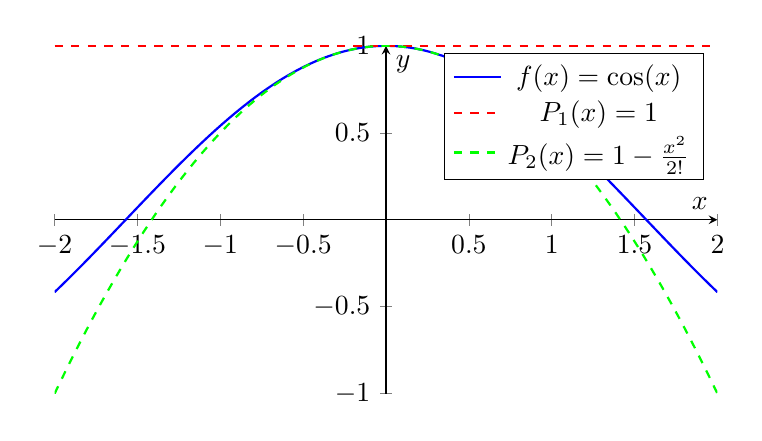
\begin{tikzpicture}
\begin{axis}[
    axis lines = middle,
    xlabel = \(x\),
    ylabel = \(y\),
    domain=-2:2,
    samples=100,
    width=10cm,
    height=6cm,
]
\addplot [blue, thick] {cos(deg(x))};
\addplot [red, thick, dashed] {1};
\addplot [green, thick, dashed] {1 - x^2/2};
\legend{\(f(x) = \cos(x)\), \(P_1(x) = 1\), \(P_2(x) = 1 - \frac{x^2}{2!}\)}
\end{axis}
\end{tikzpicture}
\end{center}

\subsection*{Error Analysis}
The error in the local linear approximation is given by:
\[ R_1(x) = f(x) - L(x) \]
For the quadratic approximation, the error term is:
\[ R_2(x) = f(x) - Q(x) \]
For Taylor polynomials, the remainder term (Lagrange form) is:
\[ R_n(x) = \frac{f^{(n+1)}(\xi)}{(n+1)!}(x - x_0)^{n+1} \]
where \( \xi \) is some point in the interval between \( x \) and \( x_0 \).

\subsection*{Convergence of Taylor Series}
The convergence of a Taylor series is a fundamental aspect of its utility in approximating functions. The Taylor series for \( f(x) \) converges to \( f(x) \) if the remainder term \( R_n(x) \) approaches zero as \( n \) approaches infinity. This can be expressed as:
\[ \lim_{n \to \infty} R_n(x) = 0 \]

\subsubsection*{Estimating the \( n \)-th Remainder}
The \( n \)-th remainder term \( R_n(x) \) in the Taylor series is given by the Lagrange form:
\[ R_n(x) = \frac{f^{(n+1)}(\xi)}{(n+1)!}(x - x_0)^{n+1} \]
where \( \xi \) is some point in the interval between \( x \) and \( x_0 \). Estimating this remainder is crucial for understanding the accuracy of the approximation.

\subsubsection*{Approximating Trigonometric Functions}
For trigonometric functions like \( \sin(x) \) and \( \cos(x) \), the Taylor series can be particularly effective. For example, the Taylor series for \( \cos(x) \) centered at \( x_0 = 0 \) is:
\[ \cos(x) = \sum_{k=0}^{\infty} \frac{(-1)^k}{(2k)!} x^{2k} \]
The remainder term helps in determining how many terms are needed for a desired accuracy.

\subsubsection*{Roundoff and Truncation Error}
When using Taylor series in numerical computations, two types of errors can occur: roundoff error and truncation error. Roundoff error arises from the finite precision of computer arithmetic, while truncation error results from approximating an infinite series by a finite number of terms. Understanding and minimizing these errors is essential for accurate computations.

\subsubsection*{Approximating Exponential Functions}
The exponential function \( e^x \) has a well-known Taylor series:
\[ e^x = \sum_{k=0}^{\infty} \frac{x^k}{k!} \]
This series converges for all \( x \), and the remainder term can be used to estimate the error in the approximation.

\subsubsection*{Approximating Logarithms}
The natural logarithm \( \ln(1+x) \) can be approximated using its Taylor series:
\[ \ln(1+x) = \sum_{k=1}^{\infty} \frac{(-1)^{k+1}}{k} x^k \]
This series converges for \( -1 < x \leq 1 \). The remainder term provides insight into the accuracy of the approximation for a given number of terms.

\subsubsection*{Approximating \( \pi \)}
Taylor series can also be used to approximate constants like \( \pi \). For instance, the arctangent function \( \arctan(x) \) has a Taylor series:
\[ \arctan(x) = \sum_{k=0}^{\infty} \frac{(-1)^k}{2k+1} x^{2k+1} \]
By evaluating this series at specific values, one can approximate \( \pi \).

\subsubsection*{Binomial Series}
The binomial series is another important series in approximation:
\[ (1 + x)^n = \sum_{k=0}^{\infty} \binom{n}{k} x^k \]
This series converges for \( |x| < 1 \) and is useful in various applications.

\subsubsection*{Some Important Maclaurin Series}
Several functions have well-known Maclaurin series (Taylor series centered at \( x_0 = 0 \)):
\begin{itemize}
    \item \( e^x = \sum_{k=0}^{\infty} \frac{x^k}{k!} \)
    \item \( \sin(x) = \sum_{k=0}^{\infty} \frac{(-1)^k}{(2k+1)!} x^{2k+1} \)
    \item \( \cos(x) = \sum_{k=0}^{\infty} \frac{(-1)^k}{(2k)!} x^{2k} \)
    \item \( \ln(1+x) = \sum_{k=1}^{\infty} \frac{(-1)^{k+1}}{k} x^k \)
\end{itemize}
These series are fundamental in both theoretical and applied mathematics.
\subsection*{Higher-Order Approximations}
Higher-order Taylor polynomials include terms up to the \( n \)-th derivative:
\[ P_n(x) = \sum_{k=0}^{n} \frac{f^{(k)}(x_0)}{k!} (x - x_0)^k \]
\subsection*{Importance of Error Analysis}
Error analysis is important because it helps us understand how accurate our Taylor polynomial approximation is. When we use a Taylor polynomial to approximate a function, we are not using the entire infinite series, so there is always some error. By calculating this error, we can see how close our approximation is to the actual function and decide if we need a higher degree polynomial for better accuracy.

\subsubsection*{How to Calculate Error Analysis}
To find out how much error there is in a Taylor polynomial approximation, we use something called the remainder term. This term tells us the difference between the actual function and the Taylor polynomial. For an \( n \)-th degree Taylor polynomial, the remainder term is:
\[ R_n(x) = \frac{f^{(n+1)}(\xi)}{(n+1)!}(x - x_0)^{n+1} \]
where \( \xi \) is some point between \( x \) and \( x_0 \).

Steps to calculate the error:
1. Identify the function \( f(x) \) and the point \( x_0 \) where the Taylor polynomial is centered.
2. Choose the degree \( n \) of the Taylor polynomial.
3. Find the \((n+1)\)-th derivative of the function, \( f^{(n+1)}(x) \).
4. Evaluate \( f^{(n+1)}(\xi) \) for some \( \xi \) between \( x \) and \( x_0 \).
5. Plug these values into the remainder term formula to get \( R_n(x) \).

By looking at the remainder term, we can judge how good our Taylor polynomial is and whether it is accurate enough for what we need.

\subsubsection*{Example: Approximating \( e^x \) using Taylor Series}

Let's consider the function \( f(x) = e^x \) and approximate it using Taylor series centered at \( x_0 = 0 \).

1. Identify the function \( f(x) = e^x \) and the point \( x_0 = 0 \).
2. The derivatives of \( f(x) = e^x \) are all \( f^{(k)}(x) = e^x \), and at \( x_0 = 0 \), \( f^{(k)}(0) = 1 \) for all \( k \).

The Taylor series for \( f(x) = e^x \) centered at \( x_0 = 0 \) is:
\[ P_n(x) = \sum_{k=0}^{n} \frac{f^{(k)}(0)}{k!} x^k = \sum_{k=0}^{n} \frac{x^k}{k!} \]

For example, the first few Taylor polynomials are:
\begin{itemize}
\item \( P_0(x) = 1 \)
\item \( P_1(x) = 1 + x \)
\item \( P_2(x) = 1 + x + \frac{x^2}{2!} \)
\item \( P_3(x) = 1 + x + \frac{x^2}{2!} + \frac{x^3}{3!} \)
\item And so on.
\end{itemize}

Using sigma notation, the \( n \)-th Taylor polynomial for \( f(x) = e^x \) centered at \( x_0 = 0 \) is:
\[ P_n(x) = \sum_{k=0}^{n} \frac{x^k}{k!} \]

\subsubsection*{Error Analysis for \( e^x \)}

To find the error in the Taylor polynomial approximation of \( e^x \), we use the remainder estimation theorem. The remainder term \( R_n(x) \) for the Taylor series is given by:
\[ R_n(x) = \frac{f^{(n+1)}(\xi)}{(n+1)!} (x - x_0)^{n+1} \]
where \( \xi \) is some point between \( x \) and \( x_0 \).

For \( f(x) = e^x \) centered at \( x_0 = 0 \), the \((n+1)\)-th derivative is \( f^{(n+1)}(x) = e^x \). Thus, the remainder term becomes:
\[ R_n(x) = \frac{e^{\xi}}{(n+1)!} x^{n+1} \]
where \( \xi \) is some point between \( x \) and \( 0 \).

For example, if we approximate \( e^x \) using the 3rd-degree Taylor polynomial \( P_3(x) \), the error term is:
\[ R_3(x) = \frac{e^{\xi}}{4!} x^4 \]
where \( \xi \) is some point between \( x \) and \( 0 \).

By calculating this remainder term, we can estimate the error in our Taylor polynomial approximation of \( e^x \). For instance, if \( x = 0.1 \), then \( \xi \) is between \( 0 \) and \( 0.1 \), and we can bound the error as:
\[ R_3(0.1) \leq \frac{e^{0.1}}{24} (0.1)^4 \approx \frac{1.105}{24} \times 0.0001 \approx 0.0000046 \]

This shows that the error in the 3rd-degree Taylor polynomial approximation of \( e^{0.1} \) is very small.



\subsection*{Applications}
Taylor and Maclaurin polynomials are used in numerical methods, physics, engineering, and computer science for approximating functions, solving differential equations, and in algorithms for scientific computing.

\end{document}